\documentclass[aspectratio=169,10pt,compress]{beamer}

\useoutertheme{split}
\useinnertheme{rounded}
\usecolortheme{whale}
\usecolortheme{orchid}
\setbeamertemplate{blocks}[rounded]
\setbeamertemplate{navigation symbols}{}
\setbeamertemplate{page number in head/foot}[totalframenumber]
% split footline shows "i / N" (frame number / total frames) on every frame

\usepackage[T1]{fontenc}
\usepackage{lmodern}
\usepackage{listings}
\usepackage{xcolor}
\usepackage{booktabs}
\usepackage{array}
\usepackage{tikz}
\usetikzlibrary{positioning,arrows.meta,calc}

\newcolumntype{L}[1]{>{\raggedright\arraybackslash}p{#1}}

\definecolor{codebg}{RGB}{245,245,245}
\definecolor{codecomment}{RGB}{110,110,110}
\definecolor{gitred}{RGB}{240,80,50}
\definecolor{gitblue}{RGB}{40,90,160}
\definecolor{gitgreen}{RGB}{40,130,70}

\lstset{
  language=bash,
  basicstyle=\ttfamily\footnotesize,
  backgroundcolor=\color{codebg},
  commentstyle=\color{codecomment}\itshape,
  keywordstyle=\color{gitred}\bfseries,
  morekeywords={git},
  frame=single,
  rulecolor=\color{gray!40},
  columns=fullflexible,
  keepspaces=true,
  showstringspaces=false,
  breaklines=true,
  xleftmargin=4pt,
  xrightmargin=4pt,
  aboveskip=4pt,
  belowskip=4pt
}

\newcommand{\cmd}[1]{\texttt{\color{gitred}#1}}

\tikzset{
  commit/.style={circle, draw=gitblue, fill=gitblue!15, thick, minimum size=7mm,
                 inner sep=0pt, font=\scriptsize\ttfamily},
  newcommit/.style={commit, draw=gitred, fill=gitred!15},
  edge/.style={-{Stealth[length=2mm]}, thick, gray!70},
  lbl/.style={font=\scriptsize\bfseries, text=gitred},
  ref/.style={draw=gitred, thick, fill=gitred!12, rounded corners=2pt,
              font=\scriptsize\ttfamily, inner sep=2pt},
  headref/.style={ref, draw=gitblue, fill=gitblue!12},
  ptr/.style={-{Stealth[length=1.6mm]}, thick, gitred}
}

\definecolor{diffadd}{RGB}{20,120,50}
\definecolor{diffdel}{RGB}{200,40,40}

% unified-diff listings: color whole lines by their first character
\lstdefinelanguage{udiff}{
  morecomment=[f][\color{gitblue}\bfseries]{@@},
  morecomment=[f][\color{diffadd}]{+},
  morecomment=[f][\color{diffdel}]{-}
}
\lstdefinestyle{diff}{language=udiff, commentstyle={}, escapechar=\&}

\tikzset{
  snap/.style={draw=gitblue, thick, fill=gitblue!10, rounded corners=3pt,
               minimum width=1.3cm, minimum height=0.9cm, font=\small},
  delta/.style={-{Stealth[length=2mm]}, thick, gitred},
  dlbl/.style={font=\small, text=gitred, fill=white, inner sep=1pt},
  box/.style={draw, rounded corners, thick, minimum width=3.1cm, minimum height=1.1cm,
              align=center, font=\small},
  obj/.style={draw, rounded corners, thick, minimum width=1.9cm, minimum height=0.75cm,
              align=center, font=\scriptsize}
}

\title{Git as Diff}
\subtitle{Snapshots Stored, Diffs Everywhere}
\author[Bingol]{Haluk O. Bingol}

\institute[FCIS]{
    Faculty of Computer and Information Sciences\\
    Yeditepe University
}
\date{}

\begin{document}

% ~~~~~~~~~~~~~~~~~~~~~~~~~~~~~~~~~~~~~~ V
\begin{frame}[t,fragile]
  \titlepage
\end{frame}
% ~~~~~~~~~~~~~~~~~~~~~~~~~~~~~~~~~~~~~~ A

% ~~~~~~~~~~~~~~~~~~~~~~~~~~~~~~~~~~~~~~ V
\begin{frame}[t,fragile] \frametitle{Outline}
  \begin{columns}[T]
    \begin{column}{0.5\textwidth}
      \tableofcontents[sections={1-4}]
    \end{column}
    \begin{column}{0.5\textwidth}
      \tableofcontents[sections={5-8}]
    \end{column}
  \end{columns}
\end{frame}
% ~~~~~~~~~~~~~~~~~~~~~~~~~~~~~~~~~~~~~~ A

% ~~~~~~~~~~~~~~~~~~~~~~~~~~~~~~~~~~~~~~ V
\begin{frame}[t,fragile] \frametitle{The one idea}
  \vspace{1em}
  \begin{center}
    \Large Git \textbf{stores snapshots} but \textbf{thinks in diffs}.
  \end{center}
  \vspace{1em}

  \begin{itemize}
    \item Every commit is a \emph{complete} picture of the project
    \item But almost every command \textbf{computes} a diff between two snapshots,
          \textbf{moves} it, or \textbf{re-applies} it somewhere else
    \item \cmd{add}, \cmd{commit}, \cmd{merge}, \cmd{rebase}, \cmd{cherry-pick},
          \cmd{revert}, \cmd{stash}: all diff operations
  \end{itemize}

  \vspace{1em}
  \begin{block}{Why learn Git this way?}
    Instead of memorizing 20 commands, you learn one concept and a few rules for combining it.
    Then you can predict what a command will do before running it.
  \end{block}
\end{frame}
% ~~~~~~~~~~~~~~~~~~~~~~~~~~~~~~~~~~~~~~ A

% ~~~~~~~~~~~~~~~~~~~~~~~~~~~~~~~~~~~~~~ V
\section[Diffs]{What Is a Diff?}
% ~~~~~~~~~~~~~~~~~~~~~~~~~~~~~~~~~~~~~~ A

% ~~~~~~~~~~~~~~~~~~~~~~~~~~~~~~~~~~~~~~ V
\begin{frame}[t,fragile] \frametitle{A diff is the change between two states}
  \begin{center}
  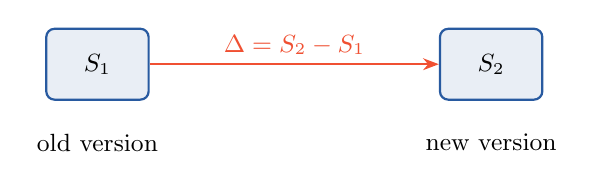
\begin{tikzpicture}
    \node[snap] (s1) at (0,0) {$S_1$};
    \node[snap] (s2) at (5,0) {$S_2$};
    \draw[delta] (s1) -- node[dlbl, above=2pt]{$\Delta = S_2 - S_1$} (s2);
    \node[font=\small, below=3mm of s1] {old version};
    \node[font=\small, below=3mm of s2] {new version};
  \end{tikzpicture}
  \end{center}

  \begin{itemize}
    \item \textbf{Compute} a diff: compare two versions line by line
    \item \textbf{Apply} a diff: $S_1 + \Delta = S_2$
    \item \textbf{Invert} a diff: swap the \texttt{+} and \texttt{-} lines, so $S_2 - \Delta = S_1$
  \end{itemize}

  \begin{columns}[T]
    \begin{column}{0.48\textwidth}
\begin{lstlisting}
diff -u old.py new.py   # Unix
git diff                # Git
\end{lstlisting}
    \end{column}
    \begin{column}{0.48\textwidth}
      \small A diff is usually much smaller than the files it connects:
      it lists only what changed, plus a few lines of context.
    \end{column}
  \end{columns}
\end{frame}
% ~~~~~~~~~~~~~~~~~~~~~~~~~~~~~~~~~~~~~~ A

% ~~~~~~~~~~~~~~~~~~~~~~~~~~~~~~~~~~~~~~ V
\begin{frame}[t,fragile] \frametitle{Reading a unified diff}
  \begin{columns}[T]
    \begin{column}{0.56\textwidth}
\begin{lstlisting}[style=diff]
diff --git a/grades.py b/grades.py
&\textcolor{gray}{-{}-{}- a/grades.py}&
&\textcolor{gray}{+++ b/grades.py}&
@@ -5,4 +5,5 @@ def average(grades):
     """Return the mean grade."""
-    total = sum(grades)
-    return total / len(grades)
+    if not grades:
+        return None
+    return sum(grades) / len(grades)
 
\end{lstlisting}
    \end{column}
    \begin{column}{0.41\textwidth}
      \small
      \begin{itemize}
        \item \texttt{-{}-{}-} / \texttt{+++}: old and new file
        \item \texttt{@@ -5,4 +5,5 @@}: a \textbf{hunk}: 4 lines from line 5 of the old file
              become 5 lines from line 5 of the new file
        \item \textcolor{diffdel}{\texttt{-} line}: removed
        \item \textcolor{diffadd}{\texttt{+} line}: added
        \item space: unchanged \textbf{context}, used to find the right place
      \end{itemize}
    \end{column}
  \end{columns}

  \vspace{0.5em}
  \begin{block}{Note}
    Diffs are line-based. Changing one character replaces the whole line:
    one \texttt{-} line and one \texttt{+} line.
  \end{block}
\end{frame}
% ~~~~~~~~~~~~~~~~~~~~~~~~~~~~~~~~~~~~~~ A

% ~~~~~~~~~~~~~~~~~~~~~~~~~~~~~~~~~~~~~~ V
\section[3 States]{Three Snapshots, Three Diffs}
% ~~~~~~~~~~~~~~~~~~~~~~~~~~~~~~~~~~~~~~ A

% ~~~~~~~~~~~~~~~~~~~~~~~~~~~~~~~~~~~~~~ V
\begin{frame}[t,fragile] \frametitle{Three versions of your project at any moment}
  \begin{center}
  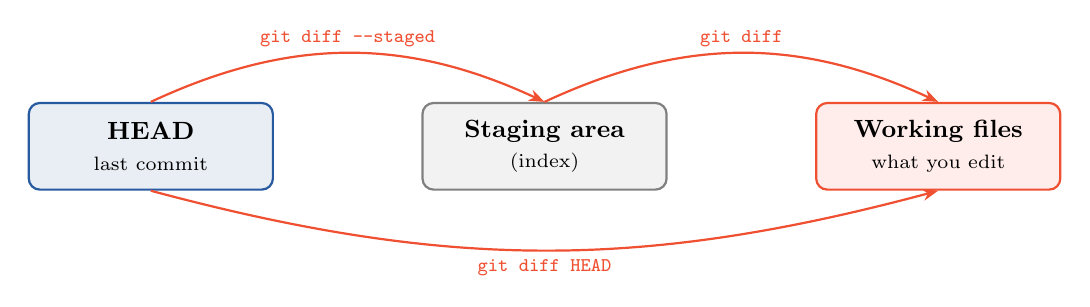
\begin{tikzpicture}
    \node[box, draw=gitblue, fill=gitblue!10] (h) at (0,0) {\textbf{HEAD}\\ \scriptsize last commit};
    \node[box, draw=gray, fill=gray!10] (i) at (5,0) {\textbf{Staging area}\\ \scriptsize (index)};
    \node[box, draw=gitred, fill=gitred!10] (w) at (10,0) {\textbf{Working files}\\ \scriptsize what you edit};
    \draw[delta] (h.north) to[bend left=25] node[dlbl, above=1pt, font=\scriptsize\ttfamily]{git diff --staged} (i.north);
    \draw[delta] (i.north) to[bend left=25] node[dlbl, above=1pt, font=\scriptsize\ttfamily]{git diff} (w.north);
    \draw[delta] (h.south) to[bend right=15] node[dlbl, below=2pt, font=\scriptsize\ttfamily]{git diff HEAD} (w.south);
  \end{tikzpicture}
  \end{center}

  \small
  \begin{tabular}{@{}L{0.28\textwidth}L{0.34\textwidth}L{0.3\textwidth}@{}}
    \toprule
    \textbf{Command} & \textbf{Diff between} & \textbf{Meaning} \\
    \midrule
    \cmd{git diff} & staging area $\rightarrow$ working files & changes not yet staged \\
    \cmd{git diff --staged} & HEAD $\rightarrow$ staging area & what \cmd{commit} will record \\
    \cmd{git diff HEAD} & HEAD $\rightarrow$ working files & all your changes \\
    \bottomrule
  \end{tabular}

  \vspace{0.5em}
  \normalsize
  Note that $\Delta_{\text{HEAD}} = \Delta_{\text{staged}} + \Delta_{\text{unstaged}}$.
\end{frame}
% ~~~~~~~~~~~~~~~~~~~~~~~~~~~~~~~~~~~~~~ A

% ~~~~~~~~~~~~~~~~~~~~~~~~~~~~~~~~~~~~~~ V
\begin{frame}[t,fragile] \frametitle{Everyday commands move diffs between the three}
  \small
  \begin{tabular}{@{}L{0.3\textwidth}L{0.62\textwidth}@{}}
    \toprule
    \textbf{Command} & \textbf{What happens to the diff} \\
    \midrule
    \cmd{git add file} & the unstaged diff of \texttt{file} moves into the staging area \\
    \cmd{git add -p} & only the \emph{hunks} you choose move \\
    \cmd{git commit} & the staged diff becomes a new snapshot; HEAD moves to it \\
    \cmd{git restore --staged file} & the staged diff moves back to unstaged \\
    \cmd{git restore file} & the unstaged diff is \textbf{thrown away} \\
    \cmd{git commit --amend} & the staged diff is added to the last commit's diff \\
    \bottomrule
  \end{tabular}

  \vspace{0.8em}
  \normalsize
\begin{lstlisting}
git diff --stat           # summary: files changed, lines added/removed
git diff --staged         # always check this right before committing
\end{lstlisting}

  \begin{block}{Habit}
    Before every commit, read \cmd{git diff --staged}. It is exactly what your commit will contain.
  \end{block}
\end{frame}
% ~~~~~~~~~~~~~~~~~~~~~~~~~~~~~~~~~~~~~~ A

% ~~~~~~~~~~~~~~~~~~~~~~~~~~~~~~~~~~~~~~ V
\section[History]{History as a Chain of Diffs}
% ~~~~~~~~~~~~~~~~~~~~~~~~~~~~~~~~~~~~~~ A

% ~~~~~~~~~~~~~~~~~~~~~~~~~~~~~~~~~~~~~~ V
\begin{frame}[t,fragile] \frametitle{Every commit implies a diff}
  \begin{center}
  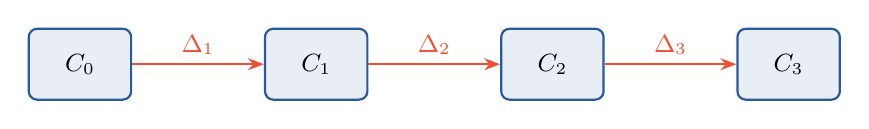
\begin{tikzpicture}
    \foreach \i/\x in {0/0,1/3,2/6,3/9} \node[snap] (c\i) at (\x,0) {$C_\i$};
    \draw[delta] (c0) -- node[dlbl, above=2pt]{$\Delta_1$} (c1);
    \draw[delta] (c1) -- node[dlbl, above=2pt]{$\Delta_2$} (c2);
    \draw[delta] (c2) -- node[dlbl, above=2pt]{$\Delta_3$} (c3);
  \end{tikzpicture}
  \end{center}

  A commit $C_i$ has a parent $C_{i-1}$, so it \emph{implies} the diff
  $\Delta_i = C_i - C_{i-1}$. Read this way:
  \[
    C_n = C_0 + \Delta_1 + \Delta_2 + \dots + \Delta_n
  \]

\begin{lstlisting}
git show a1b2c3d          # the diff of one commit (vs. its parent)
git log -p                # history as a list of diffs
git log -p -- grades.py   # only the diffs touching one file
git diff v1.0 v2.0        # sum of all diffs between two versions
\end{lstlisting}
\end{frame}
% ~~~~~~~~~~~~~~~~~~~~~~~~~~~~~~~~~~~~~~ A

% ~~~~~~~~~~~~~~~~~~~~~~~~~~~~~~~~~~~~~~ V
\begin{frame}[t,fragile] \frametitle{Branches are chains of diffs from a shared commit}
  \begin{center}
  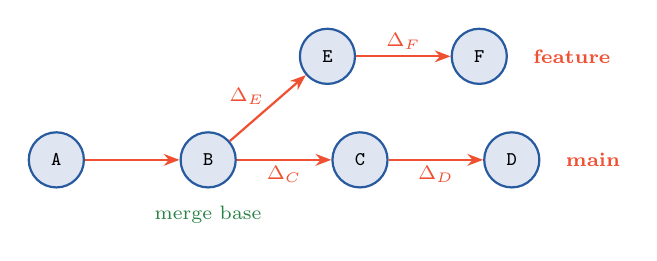
\begin{tikzpicture}[node distance=12mm]
    \node[commit] (a) {A};
    \node[commit, right=of a] (b) {B};
    \node[commit, right=of b] (c) {C};
    \node[commit, right=of c] (d) {D};
    \node[commit, above right=8mm and 10mm of b] (e) {E};
    \node[commit, right=of e] (f) {F};
    \draw[delta] (a) -- (b);
    \draw[delta] (b) -- node[dlbl, below=1pt, font=\scriptsize]{$\Delta_C$} (c);
    \draw[delta] (c) -- node[dlbl, below=1pt, font=\scriptsize]{$\Delta_D$} (d);
    \draw[delta] (b) -- node[dlbl, above left=0pt, font=\scriptsize]{$\Delta_E$} (e);
    \draw[delta] (e) -- node[dlbl, above=1pt, font=\scriptsize]{$\Delta_F$} (f);
    \node[lbl, right=2mm of d] {main};
    \node[lbl, right=2mm of f] {feature};
    \node[font=\scriptsize, text=gitgreen, below=1mm of b] {merge base};
  \end{tikzpicture}
  \end{center}

  \small
  \begin{tabular}{@{}L{0.33\textwidth}L{0.6\textwidth}@{}}
    \toprule
    \textbf{Command} & \textbf{Diff shown} \\
    \midrule
    \cmd{git diff main feature} & $F - D$: tip to tip (includes ``undoing'' $\Delta_C, \Delta_D$) \\
    \cmd{git diff main...feature} & $F - B = \Delta_E + \Delta_F$: only what \texttt{feature} added \\
    \cmd{git merge-base main feature} & $B$ \\
    \bottomrule
  \end{tabular}

  \vspace{0.5em}
  \normalsize
  The three-dot form is what a pull request shows: \emph{the diffs this branch contributes}.
\end{frame}
% ~~~~~~~~~~~~~~~~~~~~~~~~~~~~~~~~~~~~~~ A

% ~~~~~~~~~~~~~~~~~~~~~~~~~~~~~~~~~~~~~~ V
\section[Arithmetic]{Diff Arithmetic}
% ~~~~~~~~~~~~~~~~~~~~~~~~~~~~~~~~~~~~~~ A

% ~~~~~~~~~~~~~~~~~~~~~~~~~~~~~~~~~~~~~~ V
\begin{frame}[t,fragile] \frametitle{Merge: add both diffs to the base}
  \begin{columns}[T]
    \begin{column}{0.45\textwidth}
      \centering
      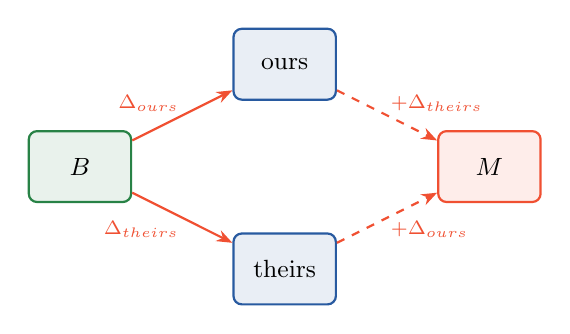
\begin{tikzpicture}
        \node[snap, draw=gitgreen, fill=gitgreen!10] (b) at (0,0) {$B$};
        \node[snap] (o) at (2.6,1.3) {ours};
        \node[snap] (t) at (2.6,-1.3) {theirs};
        \node[snap, draw=gitred, fill=gitred!10] (m) at (5.2,0) {$M$};
        \draw[delta] (b) -- node[dlbl, above left=0pt, font=\scriptsize]{$\Delta_{\text{ours}}$} (o);
        \draw[delta] (b) -- node[dlbl, below left=0pt, font=\scriptsize]{$\Delta_{\text{theirs}}$} (t);
        \draw[delta, dashed] (o) -- node[dlbl, above right=0pt, font=\scriptsize]{$+\Delta_{\text{theirs}}$} (m);
        \draw[delta, dashed] (t) -- node[dlbl, below right=0pt, font=\scriptsize]{$+\Delta_{\text{ours}}$} (m);
      \end{tikzpicture}
    \end{column}
    \begin{column}{0.52\textwidth}
      \begin{enumerate}\small
        \item Find the merge base $B$
        \item $\Delta_{\text{ours}} = \text{ours} - B$
        \item $\Delta_{\text{theirs}} = \text{theirs} - B$
        \item Apply both:
      \end{enumerate}
      \[
        M = B + \Delta_{\text{ours}} + \Delta_{\text{theirs}}
      \]
      \small
      If the two diffs touch \textbf{different lines}, the order doesn't matter and Git
      combines them automatically.
    \end{column}
  \end{columns}

  \vspace{0.5em}
  \begin{alertblock}{A conflict}
    Both diffs change the \textbf{same lines}, so there is no single way to add them.
    Git stops and asks you to write the combined result by hand.
  \end{alertblock}
\end{frame}
% ~~~~~~~~~~~~~~~~~~~~~~~~~~~~~~~~~~~~~~ A

% ~~~~~~~~~~~~~~~~~~~~~~~~~~~~~~~~~~~~~~ V
\begin{frame}[t,fragile] \frametitle{A conflict is two diffs that overlap}
  \begin{columns}[T]
    \begin{column}{0.48\textwidth}
      \small $\Delta_{\text{ours}}$ (main):
\begin{lstlisting}[style=diff]
@@ -6 +6 @@
-    total = sum(grades)
+    total = sum(grades) * weight
\end{lstlisting}
      \small $\Delta_{\text{theirs}}$ (feature):
\begin{lstlisting}[style=diff]
@@ -6 +6 @@
-    total = sum(grades)
+    total = sum(valid(grades))
\end{lstlisting}
    \end{column}
    \begin{column}{0.48\textwidth}
      \small Result, with \cmd{merge.conflictStyle zdiff3}:
\begin{lstlisting}[language={}]
<<<<<<< ours
    total = sum(grades) * weight
||||||| base
    total = sum(grades)
=======
    total = sum(valid(grades))
>>>>>>> theirs
\end{lstlisting}
    \end{column}
  \end{columns}

  \vspace{0.3em}
  \small
  The \texttt{base} section shows the line \emph{before} either diff, so you can see
  what each side meant to change. The combined intent is:
\begin{lstlisting}[language={}]
    total = sum(valid(grades)) * weight
\end{lstlisting}
\end{frame}
% ~~~~~~~~~~~~~~~~~~~~~~~~~~~~~~~~~~~~~~ A

% ~~~~~~~~~~~~~~~~~~~~~~~~~~~~~~~~~~~~~~ V
\begin{frame}[t,fragile] \frametitle{Rebase: replay the same diffs on a new base}
  \begin{columns}[T]
    \begin{column}{0.55\textwidth}
      \centering
      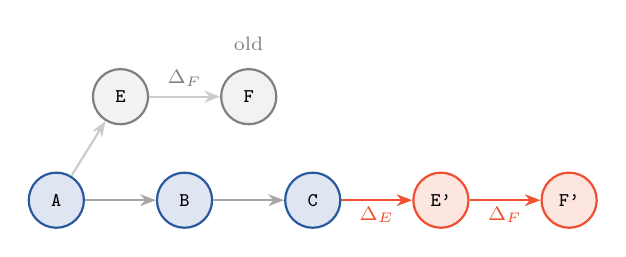
\begin{tikzpicture}[node distance=9mm]
        \node[commit] (a) {A};
        \node[commit, right=of a] (b) {B};
        \node[commit, right=of b] (c) {C};
        \node[newcommit, right=of c] (e2) {E'};
        \node[newcommit, right=of e2] (f2) {F'};
        \node[commit, draw=gray, fill=gray!10, above right=8mm and 3mm of a] (e) {E};
        \node[commit, draw=gray, fill=gray!10, right=of e] (f) {F};
        \draw[edge] (a) -- (b); \draw[edge] (b) -- (c);
        \draw[edge, gray!40] (a) -- (e);
        \draw[edge, gray!40] (e) -- node[above, font=\scriptsize, text=gray]{$\Delta_F$} (f);
        \draw[delta] (c) -- node[dlbl, below=1pt, font=\scriptsize]{$\Delta_E$} (e2);
        \draw[delta] (e2) -- node[dlbl, below=1pt, font=\scriptsize]{$\Delta_F$} (f2);
        \node[font=\scriptsize, text=gray, above=1mm of f] {old};
      \end{tikzpicture}
    \end{column}
    \begin{column}{0.42\textwidth}
      \small
      \cmd{git rebase main} on \texttt{feature}:
      \begin{enumerate}
        \item Extract the diffs $\Delta_E, \Delta_F$
        \item Start from the tip of \texttt{main}
        \item Apply them in order:\\
              $E' = C + \Delta_E$\\
              $F' = E' + \Delta_F$
      \end{enumerate}
    \end{column}
  \end{columns}

  \vspace{0.5em}
  \begin{block}{Why rebased commits get new hashes}
    The \emph{diffs} are the same, but the \emph{snapshots} are different
    ($C + \Delta_E \neq A + \Delta_E$). A commit's hash comes from its snapshot and parent,
    so $E'$ and $F'$ are new commits. That's why rewriting shared history hurts.
  \end{block}
\end{frame}
% ~~~~~~~~~~~~~~~~~~~~~~~~~~~~~~~~~~~~~~ A

% ~~~~~~~~~~~~~~~~~~~~~~~~~~~~~~~~~~~~~~ V
\begin{frame}[t,fragile] \frametitle{Cherry-pick, revert and stash}
  \begin{columns}[T]
    \begin{column}{0.32\textwidth}
      \textbf{Cherry-pick}\\[2pt]
      apply one commit's diff here
      \[ \text{new} = \text{HEAD} + \Delta_F \]
\begin{lstlisting}
git cherry-pick F
\end{lstlisting}
    \end{column}
    \begin{column}{0.32\textwidth}
      \textbf{Revert}\\[2pt]
      apply the \emph{inverse} diff
      \[ \text{new} = \text{HEAD} - \Delta_F \]
\begin{lstlisting}
git revert F
\end{lstlisting}
    \end{column}
    \begin{column}{0.32\textwidth}
      \textbf{Stash}\\[2pt]
      set your diff aside, re-apply later
      \[ \text{files} = \text{HEAD} + \Delta_{\text{wip}} \]
\begin{lstlisting}
git stash      # save, remove
git stash pop  # re-apply
\end{lstlisting}
    \end{column}
  \end{columns}

  \vspace{0.8em}
  \begin{itemize}
    \item All three can \textbf{conflict}, for the same reason as merge: the diff was made
          against one snapshot and is being applied to a different one
    \item Revert never rewrites history: it adds a new commit whose diff cancels the old one.
          That's why it is safe on shared branches
    \item \cmd{git stash show -p} shows the saved diff
  \end{itemize}
\end{frame}
% ~~~~~~~~~~~~~~~~~~~~~~~~~~~~~~~~~~~~~~ A

% ~~~~~~~~~~~~~~~~~~~~~~~~~~~~~~~~~~~~~~ V
\begin{frame}[t,fragile] \frametitle{A little patch algebra}
  \begin{itemize}
    \item \textbf{Composition:} $\Delta_{A \to C} = \Delta_{A \to B} + \Delta_{B \to C}$\\
          \small (\cmd{git diff A C} equals the diffs of all commits in between, combined)
    \item \textbf{Inverse:} $\Delta + (-\Delta) = 0$\\
          \small (a commit followed by its revert changes nothing)
    \item \textbf{Commuting:} if $\Delta_1$ and $\Delta_2$ touch different lines,
          $\Delta_1 + \Delta_2 = \Delta_2 + \Delta_1$\\
          \small (this is why most merges, rebases and cherry-picks just work)
    \item \textbf{Context-dependent:} a diff is written against a specific snapshot.
          Applied elsewhere, it may not fit\\
          \small (Git uses the context lines to find the spot; if they don't match, you get a conflict)
  \end{itemize}

  \vspace{0.5em}
  \begin{block}{The takeaway}
    Git's operations are ``add these diffs to that snapshot''. They fail only
    when two diffs don't commute, and that's exactly what a conflict is.
  \end{block}
\end{frame}
% ~~~~~~~~~~~~~~~~~~~~~~~~~~~~~~~~~~~~~~ A

% ~~~~~~~~~~~~~~~~~~~~~~~~~~~~~~~~~~~~~~ V
\section[Search]{Searching Through Diffs}
% ~~~~~~~~~~~~~~~~~~~~~~~~~~~~~~~~~~~~~~ A

% ~~~~~~~~~~~~~~~~~~~~~~~~~~~~~~~~~~~~~~ V
\begin{frame}[t,fragile] \frametitle{History is searchable because every commit has a diff}
\begin{lstlisting}
git log -S "calculate_gpa"      # diffs that add or remove this string
git log -G "def .*gpa"          # diffs whose changed lines match a regex
git log -p --follow grades.py   # every diff to one file, across renames
git blame grades.py             # which commit's diff last touched each line
git bisect run ./test.sh        # binary search for the diff that broke tests
\end{lstlisting}

  \vspace{0.3em}
  \textbf{A diff of diffs:} after a rebase, did your commits change?
\begin{lstlisting}
git range-diff main feature@{1} feature   # old series vs. new series
\end{lstlisting}
  \small \cmd{range-diff} pairs each old commit with its rebased version and shows how their
  \emph{diffs} differ. Reviewers use it to see what changed between two versions of a PR.
\end{frame}
% ~~~~~~~~~~~~~~~~~~~~~~~~~~~~~~~~~~~~~~ A

% ~~~~~~~~~~~~~~~~~~~~~~~~~~~~~~~~~~~~~~ V
\section[Patches]{Diffs Outside Git: Patches}
% ~~~~~~~~~~~~~~~~~~~~~~~~~~~~~~~~~~~~~~ A

% ~~~~~~~~~~~~~~~~~~~~~~~~~~~~~~~~~~~~~~ V
\begin{frame}[t,fragile] \frametitle{A diff saved to a file is a patch}
\begin{lstlisting}
# a plain patch: just the diff
git diff > fix.patch
git apply --check fix.patch      # would it apply cleanly?
git apply fix.patch              # apply it to the working files

# a commit as an e-mail: diff + author + message
git format-patch -3              # last 3 commits -> 0001-*.patch, 0002-*.patch, ...
git am 0001-*.patch              # apply as commits, keeping author and message

# classic Unix tools, older than Git
diff -u old.py new.py > p.patch
patch old.py < p.patch
\end{lstlisting}

  \begin{block}{Patches by e-mail}
    Before pull requests existed, projects shared work by mailing patches.
    The Linux kernel still does: \texttt{format-patch} and \texttt{am} were built for it.
  \end{block}
\end{frame}
% ~~~~~~~~~~~~~~~~~~~~~~~~~~~~~~~~~~~~~~ A

% ~~~~~~~~~~~~~~~~~~~~~~~~~~~~~~~~~~~~~~ V
\section[Snapshots]{The Truth: Snapshots}
% ~~~~~~~~~~~~~~~~~~~~~~~~~~~~~~~~~~~~~~ A

% ~~~~~~~~~~~~~~~~~~~~~~~~~~~~~~~~~~~~~~ V
\begin{frame}[t,fragile] \frametitle{What Git actually stores}
  \begin{columns}[T]
    \begin{column}{0.55\textwidth}
      \centering
      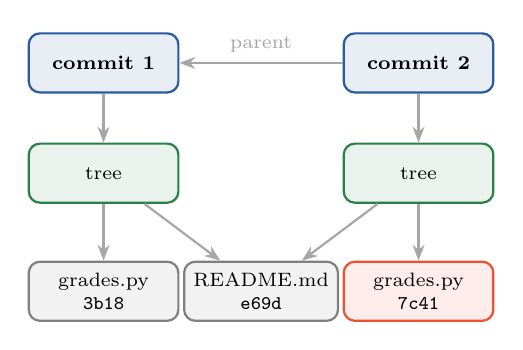
\begin{tikzpicture}
        \node[obj, draw=gitblue, fill=gitblue!10] (c1) at (0,0) {\textbf{commit 1}};
        \node[obj, draw=gitblue, fill=gitblue!10] (c2) at (4,0) {\textbf{commit 2}};
        \node[obj, draw=gitgreen, fill=gitgreen!10] (t1) at (0,-1.4) {tree};
        \node[obj, draw=gitgreen, fill=gitgreen!10] (t2) at (4,-1.4) {tree};
        \node[obj, draw=gray, fill=gray!10] (r) at (2,-2.9) {README.md\\ \texttt{e69d}};
        \node[obj, draw=gray, fill=gray!10] (g1) at (0,-2.9) {grades.py\\ \texttt{3b18}};
        \node[obj, draw=gitred, fill=gitred!10] (g2) at (4,-2.9) {grades.py\\ \texttt{7c41}};
        \draw[edge] (c2) -- node[above, font=\scriptsize]{parent} (c1);
        \draw[edge] (c1) -- (t1); \draw[edge] (c2) -- (t2);
        \draw[edge] (t1) -- (g1); \draw[edge] (t1) -- (r);
        \draw[edge] (t2) -- (r); \draw[edge] (t2) -- (g2);
      \end{tikzpicture}
    \end{column}
    \begin{column}{0.42\textwidth}
      \small
      \begin{itemize}
        \item Each commit points to a \textbf{tree}: the \emph{whole} project
        \item Files are stored as \textbf{blobs}, named by the hash of their content
        \item An unchanged file is \textbf{shared}: both trees point to the same
              \texttt{README.md} blob
        \item A changed file is a \textbf{new blob}, not a diff
      \end{itemize}
    \end{column}
  \end{columns}

  \vspace{0.5em}
  \begin{block}{So where do diffs come from?}
    \cmd{git show} compares the two trees and computes the diff \textbf{on demand},
    every time you ask.
  \end{block}
\end{frame}
% ~~~~~~~~~~~~~~~~~~~~~~~~~~~~~~~~~~~~~~ A

% ~~~~~~~~~~~~~~~~~~~~~~~~~~~~~~~~~~~~~~ V
\begin{frame}[t,fragile] \frametitle{Why snapshots, not diffs?}
  \begin{columns}[T]
    \begin{column}{0.5\textwidth}
      \textbf{Snapshots make Git fast and simple}
      \begin{itemize}\small
        \item \textbf{Checkout is direct:} read one tree; no replaying 500 diffs
        \item \textbf{Hashes are simple:} same content $\Rightarrow$ same hash,
              so integrity checks and deduplication come free
        \item \textbf{Any two versions compare:} not just neighbors
        \item \textbf{Diff algorithms can improve} without changing stored history
              (\cmd{git diff --histogram}, \cmd{--patience})
      \end{itemize}
    \end{column}
    \begin{column}{0.47\textwidth}
      \textbf{But isn't that wasteful?}
      \begin{itemize}\small
        \item Unchanged files are shared between snapshots
        \item Objects are compressed (zlib)
        \item In \textbf{pack files}, similar objects are stored as deltas of each other,
              chosen for size, not by commit order
      \end{itemize}
      \small That delta compression is a storage trick, invisible to you.
    \end{column}
  \end{columns}

  \vspace{0.5em}
  \small
  \begin{tabular}{@{}L{0.3\textwidth}L{0.62\textwidth}@{}}
    \toprule
    \textbf{System} & \textbf{What it stores} \\
    \midrule
    RCS, CVS, early SVN & diffs (deltas) between versions \\
    Git, Mercurial & snapshots, with compression underneath \\
    Darcs, Pijul & patches as the fundamental object, with a formal patch theory \\
    \bottomrule
  \end{tabular}
\end{frame}
% ~~~~~~~~~~~~~~~~~~~~~~~~~~~~~~~~~~~~~~ A

% ~~~~~~~~~~~~~~~~~~~~~~~~~~~~~~~~~~~~~~ V
\section[Summary]{Summary}
% ~~~~~~~~~~~~~~~~~~~~~~~~~~~~~~~~~~~~~~ A

% ~~~~~~~~~~~~~~~~~~~~~~~~~~~~~~~~~~~~~~ V
\begin{frame}[t,fragile] \frametitle{Git commands as diff operations}
  \small
  \begin{tabular}{@{}L{0.25\textwidth}L{0.4\textwidth}L{0.27\textwidth}@{}}
    \toprule
    \textbf{Command} & \textbf{Diff operation} & \textbf{Formula} \\
    \midrule
    \cmd{diff}, \cmd{show}, \cmd{log -p} & compute a diff & $\Delta = S_2 - S_1$ \\
    \cmd{add}, \cmd{restore} & move a diff between areas & \\
    \cmd{commit} & freeze the staged diff as a snapshot & $C = \text{HEAD} + \Delta_{\text{staged}}$ \\
    \cmd{merge} & add two diffs to their base & $M = B + \Delta_o + \Delta_t$ \\
    \cmd{rebase} & replay diffs on a new base & $E' = C + \Delta_E$ \\
    \cmd{cherry-pick} & apply one diff here & $\text{HEAD} + \Delta_F$ \\
    \cmd{revert} & apply the inverse diff & $\text{HEAD} - \Delta_F$ \\
    \cmd{stash} / \cmd{pop} & set a diff aside, re-apply it & $\text{HEAD} + \Delta_{\text{wip}}$ \\
    \cmd{log -S}, \cmd{blame}, \cmd{bisect} & search through diffs & \\
    \cmd{format-patch}, \cmd{am} & export / import diffs & \\
    \bottomrule
  \end{tabular}

  \vspace{0.8em}
  \normalsize
  \begin{block}{One sentence}
    Git \textbf{stores snapshots} but \textbf{thinks in diffs}: most commands compute a diff
    between two snapshots and apply it somewhere.
  \end{block}
\end{frame}
% ~~~~~~~~~~~~~~~~~~~~~~~~~~~~~~~~~~~~~~ A

% ~~~~~~~~~~~~~~~~~~~~~~~~~~~~~~~~~~~~~~ V
\begin{frame}[t,fragile] \frametitle{Exercises}
  \begin{enumerate}\small
    \item Edit a file, stage part of it with \cmd{git add -p}, then edit it again.
          Show that \cmd{git diff HEAD} is the sum of \cmd{git diff --staged} and \cmd{git diff}.
    \item Make three commits. Check that \cmd{git diff C0 C3} equals the three
          \cmd{git show} diffs combined.
    \item Create two branches that change \emph{different} lines of one file and merge them.
          Then repeat with the \emph{same} line. Explain the difference using $\Delta_o$ and $\Delta_t$.
    \item Rebase a two-commit branch. Compare old and new hashes, then run
          \cmd{git range-diff} to show the diffs themselves did not change.
    \item Revert a commit, then revert the revert. What is the net diff?
    \item Send a teammate a commit with \cmd{git format-patch}; they apply it with \cmd{git am}.
          Compare authors and messages in both repositories.
    \item Use \cmd{git cat-file -p} to show that an unchanged file has the \emph{same}
          blob hash in two different commits.
  \end{enumerate}

  \vspace{0.3em}
  \begin{center}
    {\Large \textbf{Questions?}}
  \end{center}
\end{frame}
% ~~~~~~~~~~~~~~~~~~~~~~~~~~~~~~~~~~~~~~ A

\end{document}
